\chapter{ITA estimation results}
\label{ap:skin_color}

\begin{figure}[hp]
     \centering
     \begin{subfigure}{0.99\textwidth}
         \centering
         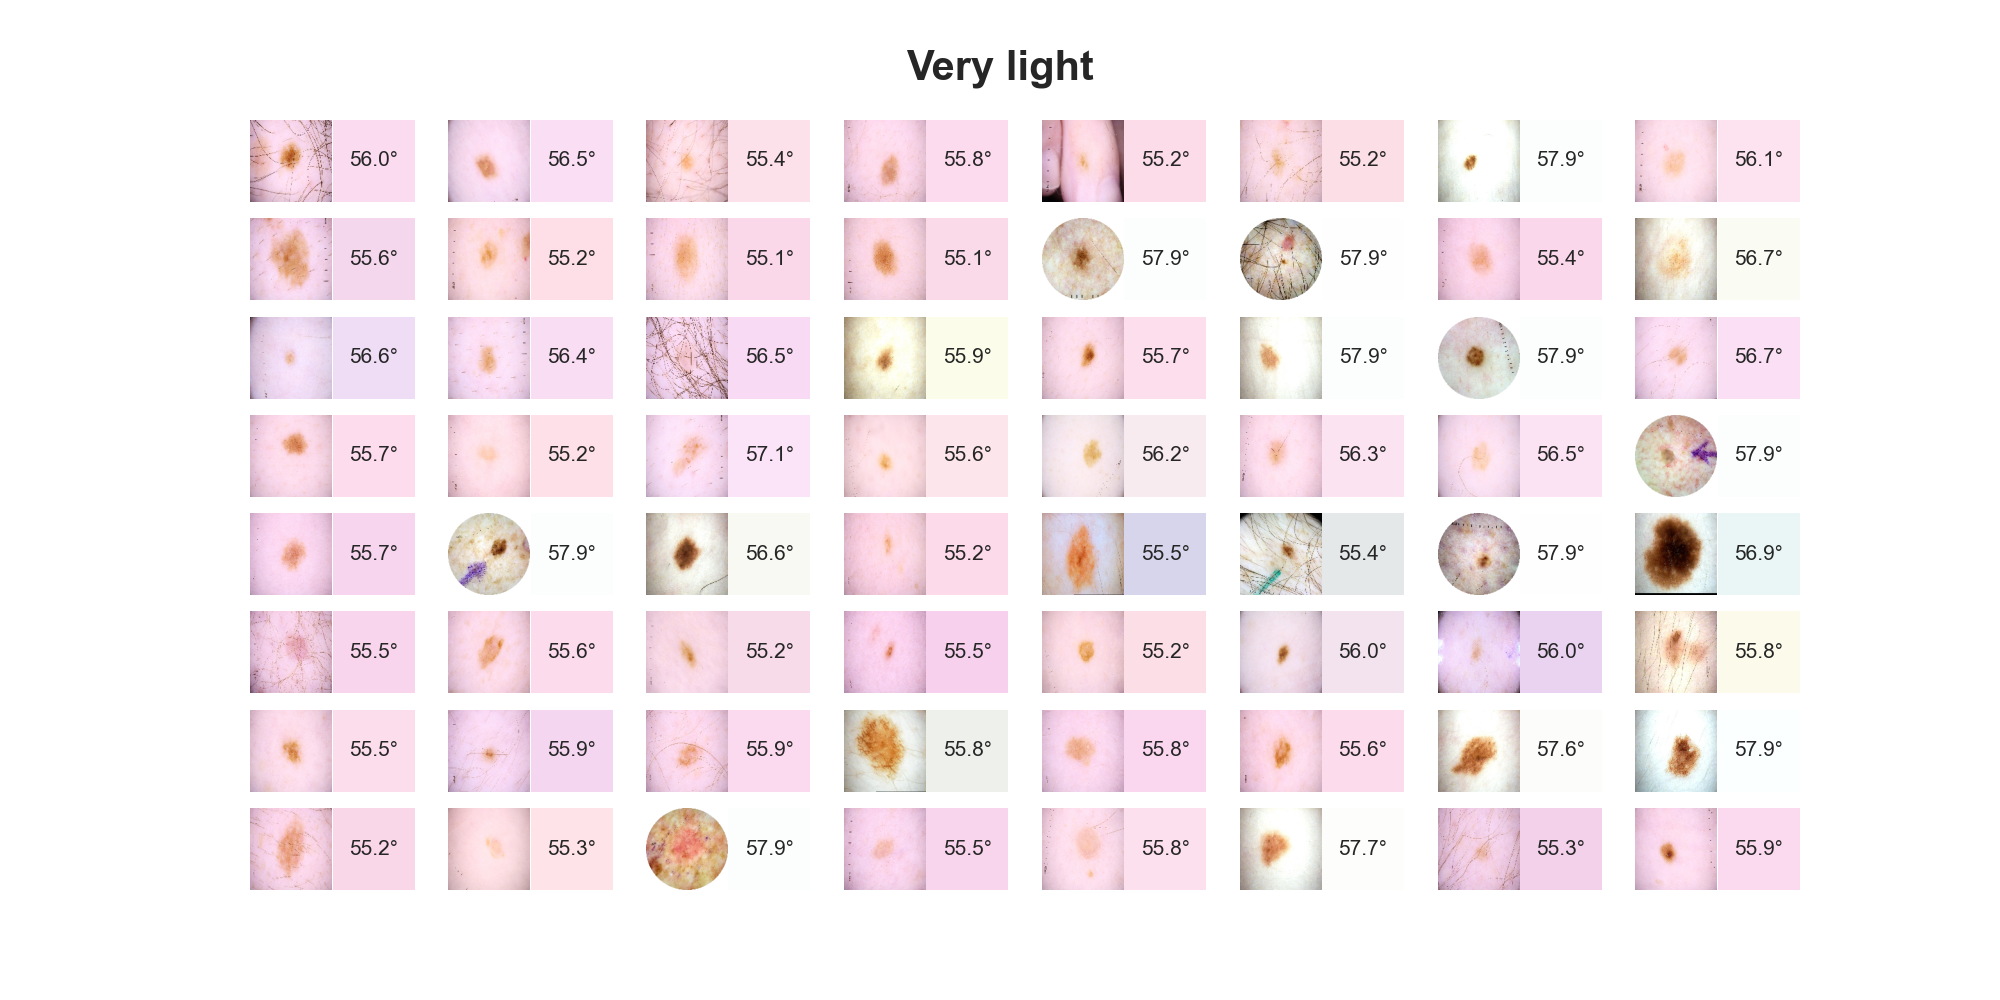
\includegraphics[width=\textwidth]{figures/eda/1 - Very light.png}
     \end{subfigure}
     \hfill
     \begin{subfigure}{0.99\textwidth}
         \centering
         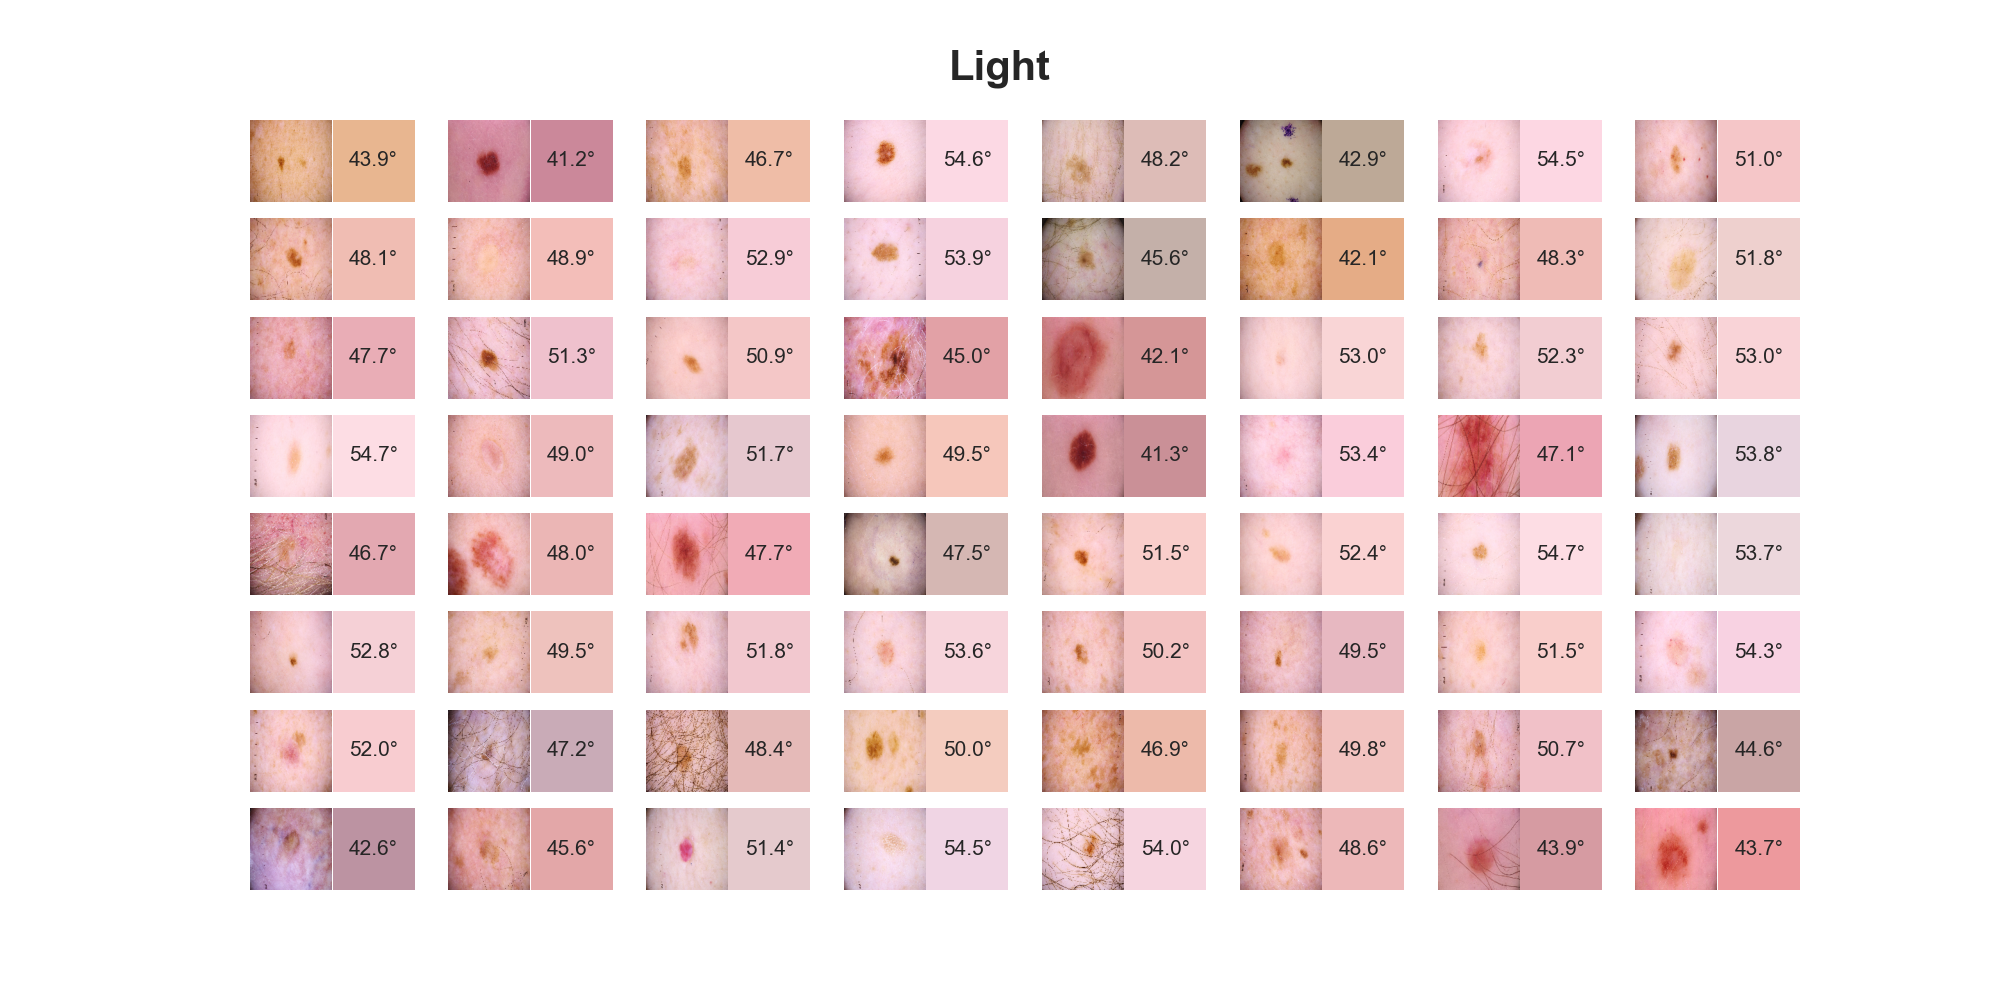
\includegraphics[width=\textwidth]{figures/eda/2- Light.png}
     \end{subfigure}
    \hfill
	\caption{Images and their estimated ITA values and dominant skin colors. Very light and light groups.}
	\label{fig:skin_colors_1}
\end{figure}



\begin{figure}[hp]
     \centering
     \begin{subfigure}{0.99\textwidth}
         \centering
         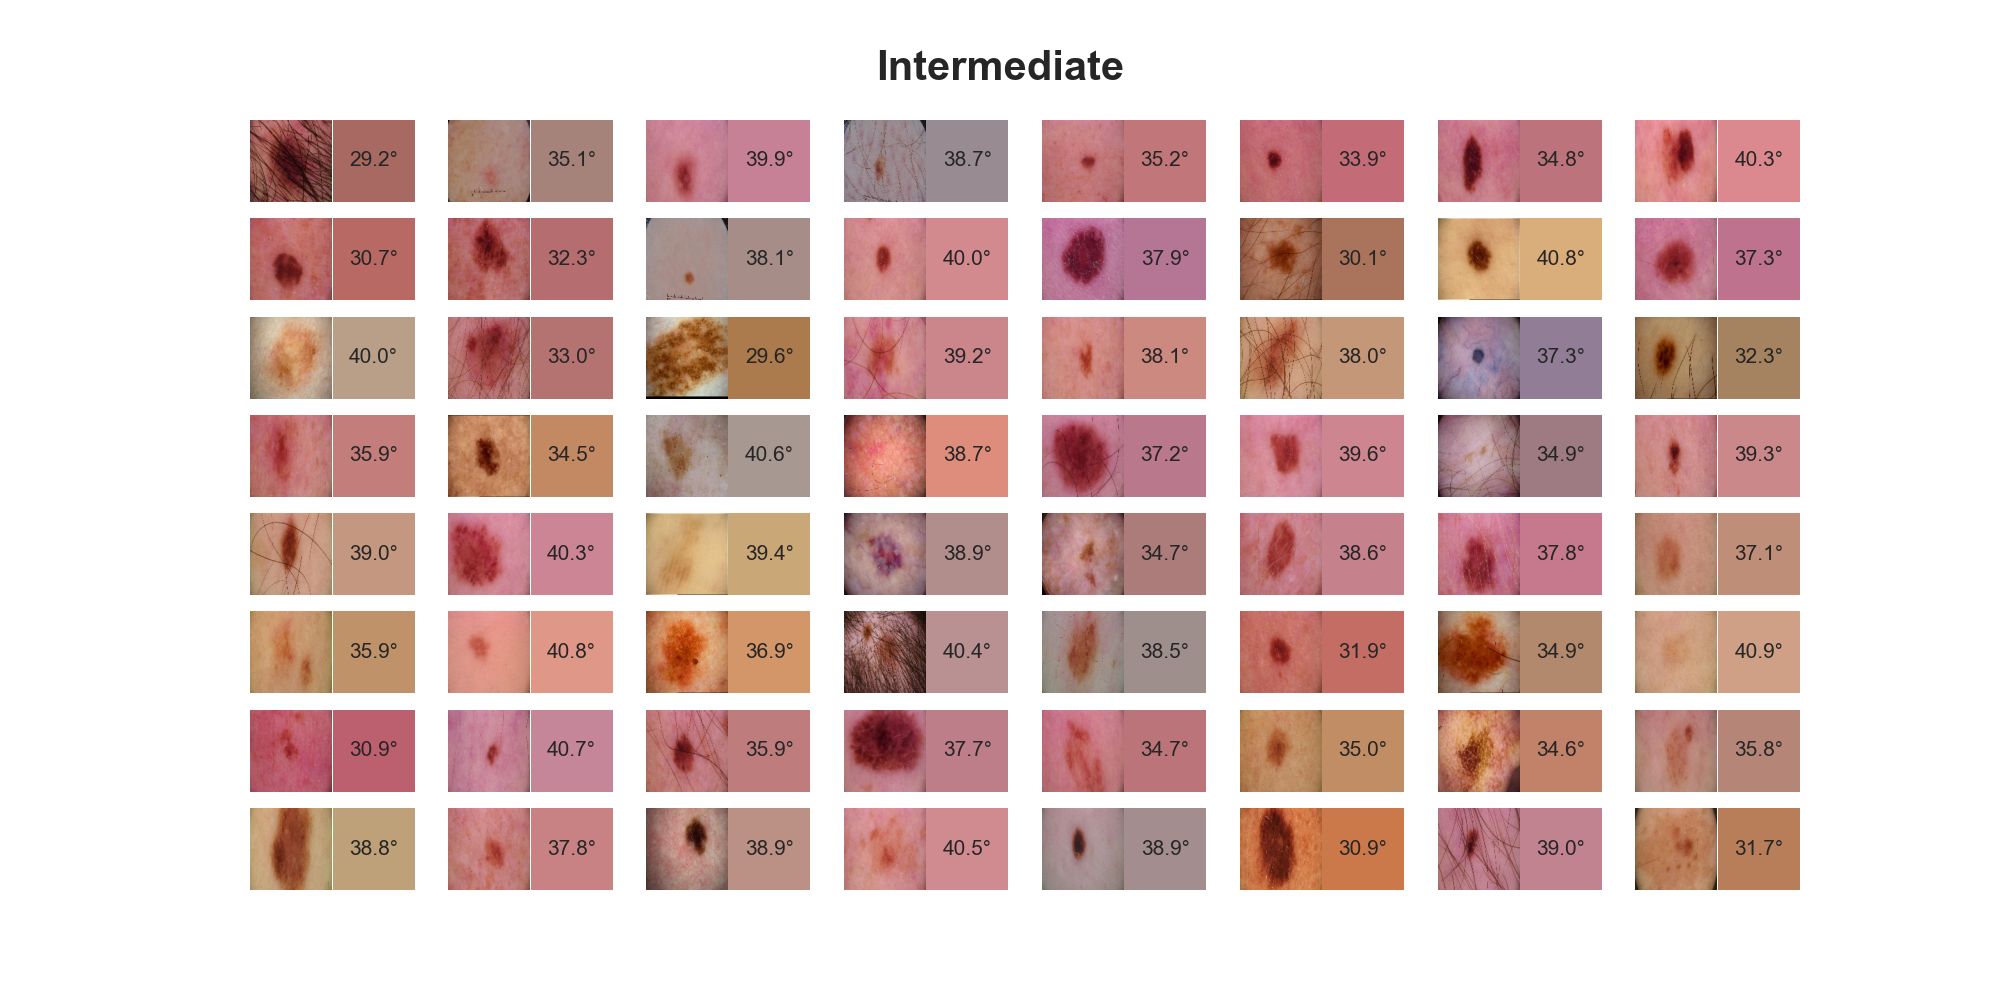
\includegraphics[width=\textwidth]{figures/eda/3 - Intermediate.png}
     \end{subfigure}
     \hfill
     \begin{subfigure}{0.99\textwidth}
         \centering
         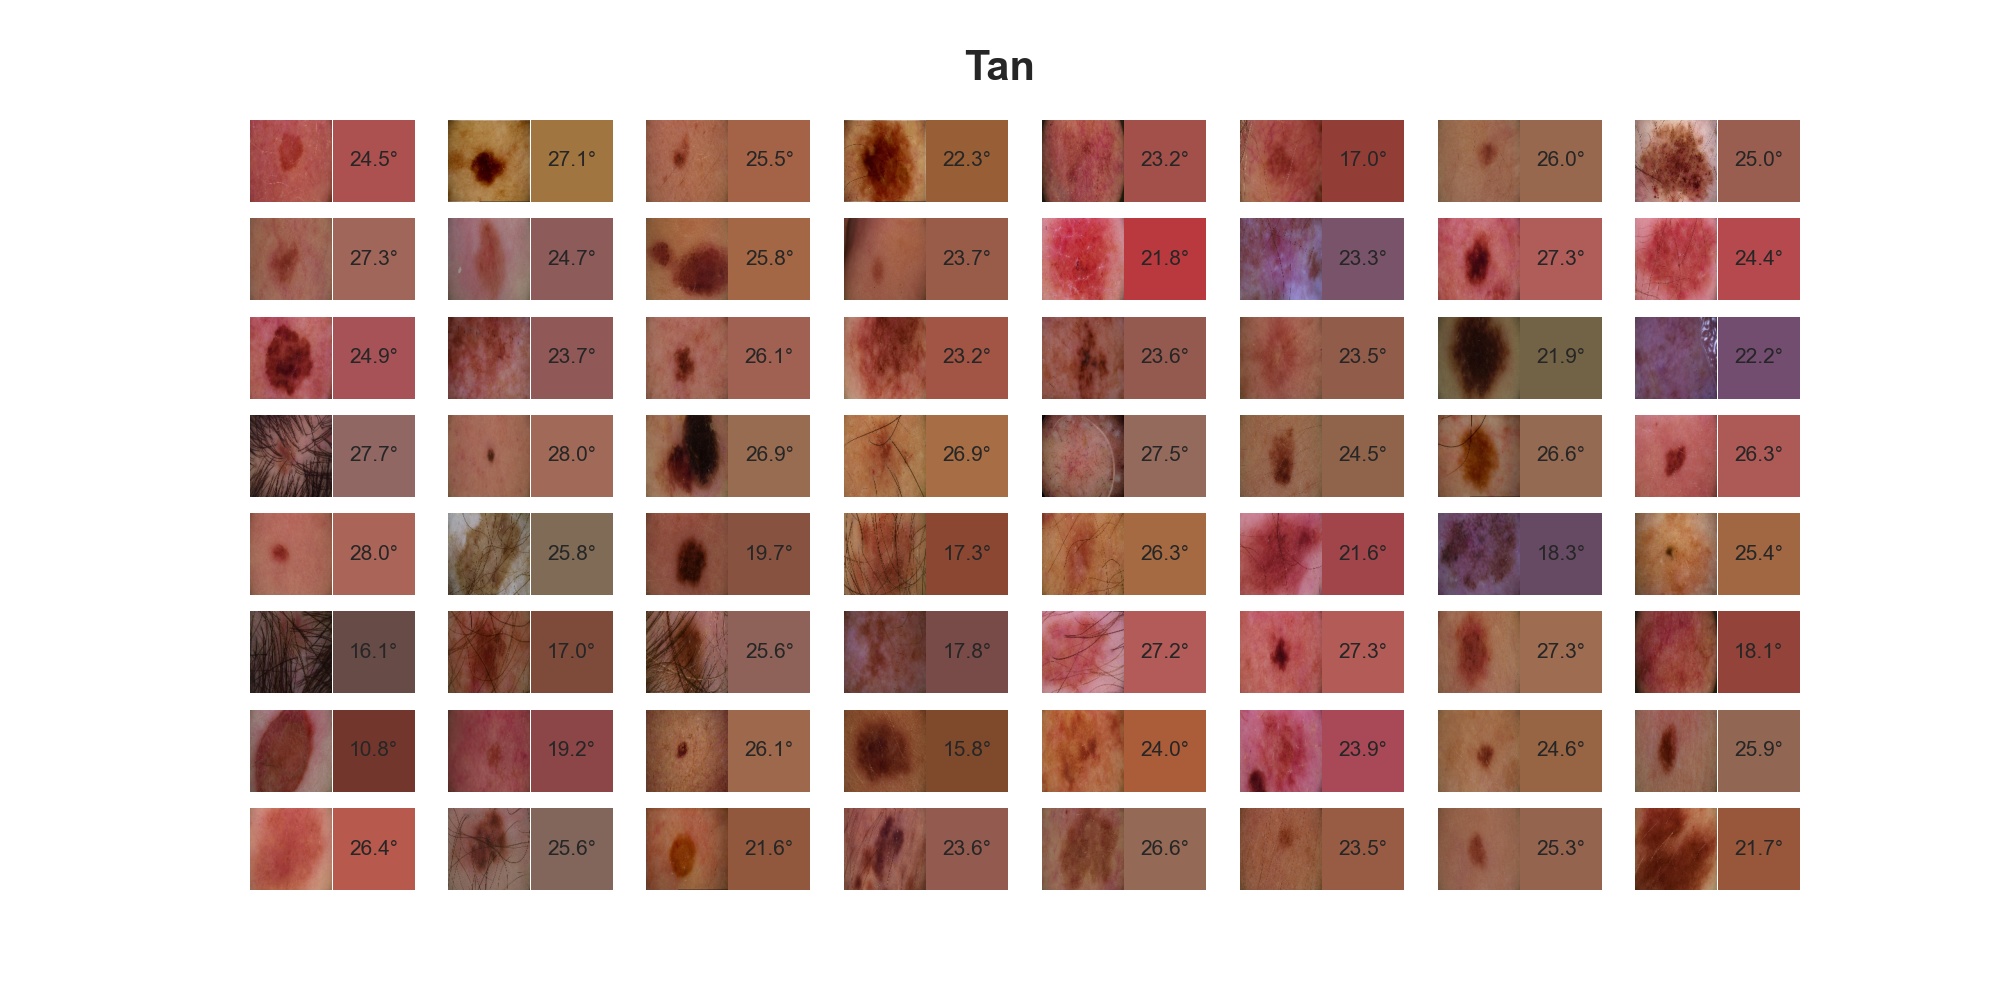
\includegraphics[width=\textwidth]{figures/eda/4 - Tan.png}
     \end{subfigure}
     \hfill
	\caption{Images and their estimated ITA values and dominant skin colors. Intermediate and tan groups.}
	\label{fig:skin_colors_2}
\end{figure}

\begin{figure}[hp]
     \centering
     \begin{subfigure}{0.99\textwidth}
         \centering
         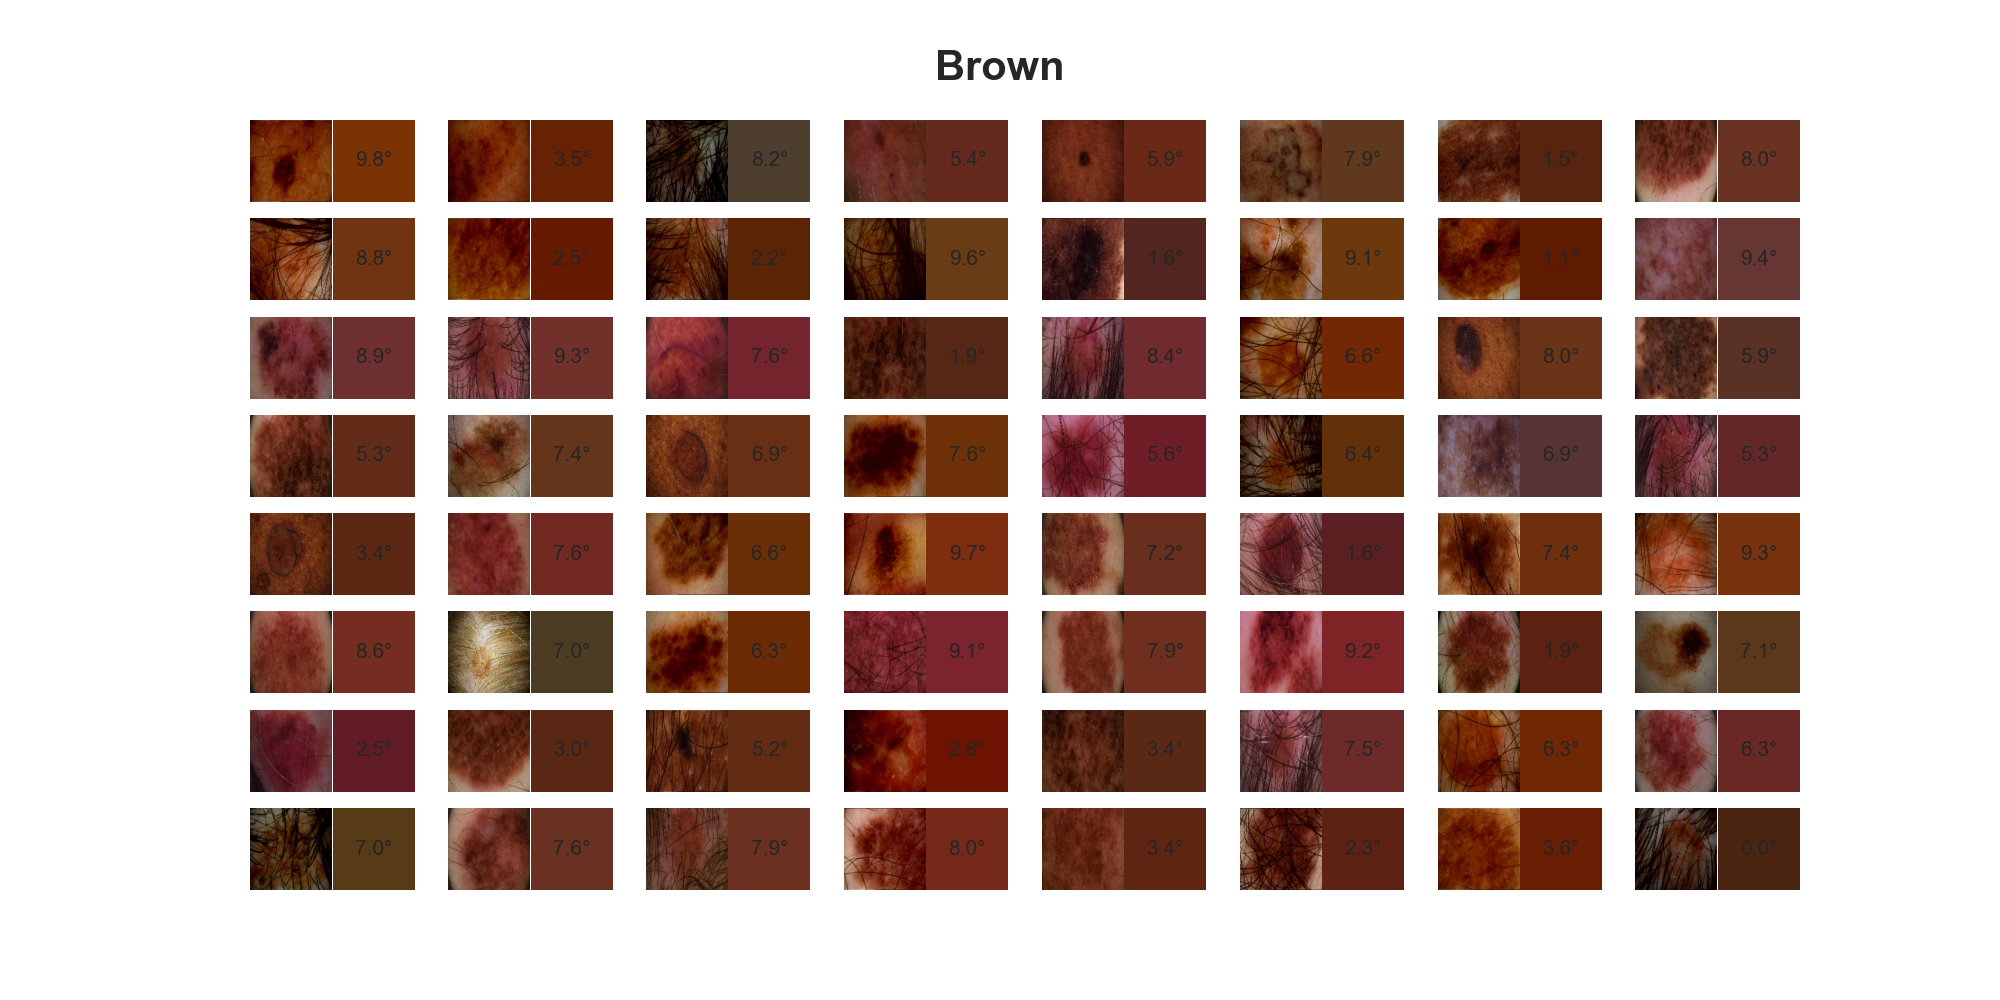
\includegraphics[width=\textwidth]{figures/eda/5 - Brown.png}
     \end{subfigure}
     \hfill
	\caption{Images and their estimated ITA values and dominant skin colors. Brown group.}
	\label{fig:skin_colors_3}
\end{figure}